 \documentclass[11pt]{article}
\usepackage[letterpaper,margin=0.7in]{geometry}
\usepackage{graphicx,amsmath,xcolor,hyperref}
\usepackage[T1]{fontenc}
\usepackage{newtxtext,newtxmath}
\definecolor{ink}{HTML}{243746}
\definecolor{wash}{HTML}{F2F5F7}
\hypersetup{colorlinks=true,urlcolor=ink}
\setlength{\parindent}{0pt}
\setlength{\parskip}{7pt}
\setlength{\fboxsep}{14pt}
\newcommand{\field}[1]{\par\vspace{5pt}{\color{ink}\bfseries #1}\par}
\begin{document}
{\small\color{ink}CHAPTER 6 \quad COMPUTATIONAL PIPELINES}\par\vspace{12pt}
\fcolorbox{ink}{white}{\begin{minipage}{\dimexpr\linewidth-2\fboxsep-2\fboxrule\relax}
{\Large\bfseries Assessment Card}\par
\textbf{Liu et al. (2020)}\par\textit{Stereochemical revision of xylogranatin F by GIAO and DU8+ NMR calculations}\par
{\small DOI: \nolinkurl{10.1002/chir.23189}}\par
\vspace{8pt}{\color{ink}\hrule}\vspace{12pt}
\begin{minipage}[t]{0.46\linewidth}\vspace{0pt}
\field{Justifications}
Publication liu\_2020\_stereochemical (DOI: 10.1002/chir.23189) is judged as \textbf{not at risk} of unreliability propagation because it cites either the paper reporting the code glitch (Neupane et al., 2019) or the addendum (Willoughby et al., 2020). Such a citation suggests that the authors were aware of the glitch and were therefore unlikely to carry its effects into their own work. This inference is defeasible: further evidence could lead us to revise the classification.
\end{minipage}\hfill
\begin{minipage}[t]{0.49\linewidth}\vspace{0pt}
\field{Reasoning visualization}
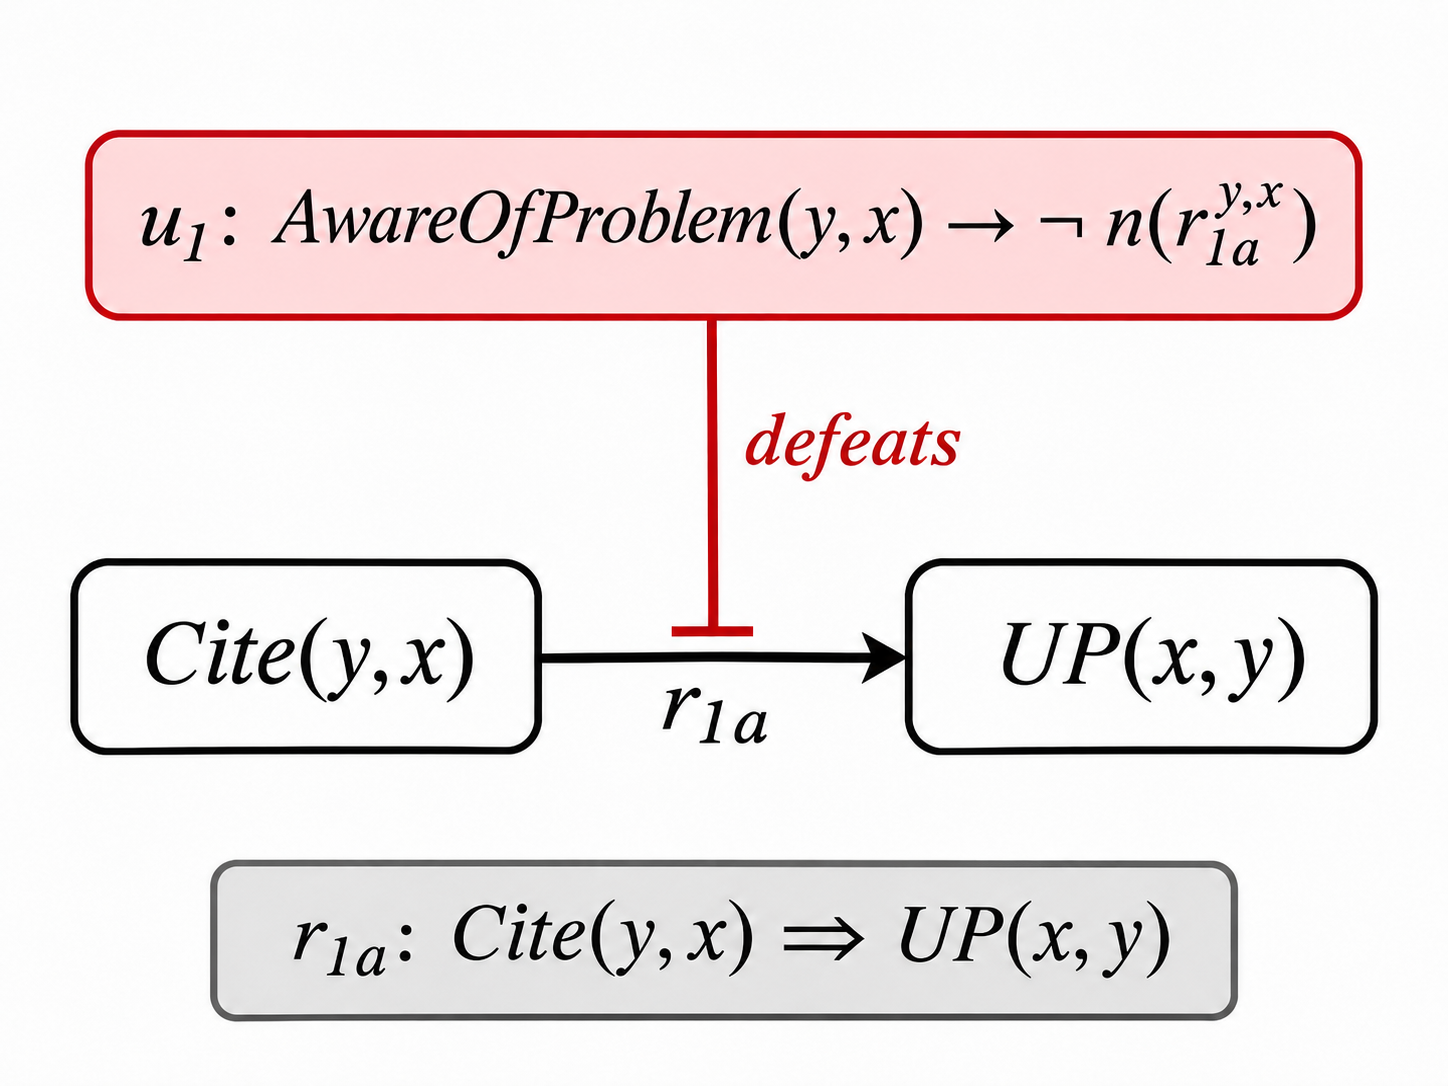
\includegraphics[width=\linewidth]{img/AwareOfProblem Defeat Diagram.png}\\[5pt]


\end{minipage}
\par\vspace{16pt}{\color{ink}\hrule}\vspace{9pt}
{\large\bfseries Final verdict: not at risk}\par

\end{minipage}}
\par\vspace{10pt}{\footnotesize Based on the annotated dataset and Chapter 6 prototype. Justifications and verdicts reproduce the saved Chapter 6 CSV results.}

\newpage
{\small\color{ink}CHAPTER 6 \quad COMPUTATIONAL PIPELINES}\par\vspace{12pt}
\fcolorbox{ink}{white}{\begin{minipage}{\dimexpr\linewidth-2\fboxsep-2\fboxrule\relax}
{\Large\bfseries Assessment Card}\par
\textbf{Jonas et al. (2022)}\par\textit{Prediction of chemical shift in NMR: A review}\par
{\small DOI: \nolinkurl{10.1002/mrc.5234}}\par
\vspace{8pt}{\color{ink}\hrule}\vspace{12pt}
\begin{minipage}[t]{0.46\linewidth}\vspace{0pt}
\field{Justifications}
Publication jonas\_2022\_prediction (DOI: 10.1002/mrc.5234) is judged as \textbf{not at risk} of unreliability propagation because it is a review article. Review articles generally discuss existing research rather than execute computational procedures such as the WJH protocol. Review status therefore provides a reason not to infer that the authors used the protocol merely because they cited it.
\end{minipage}\hfill
\begin{minipage}[t]{0.49\linewidth}\vspace{0pt}
\field{Reasoning visualization}
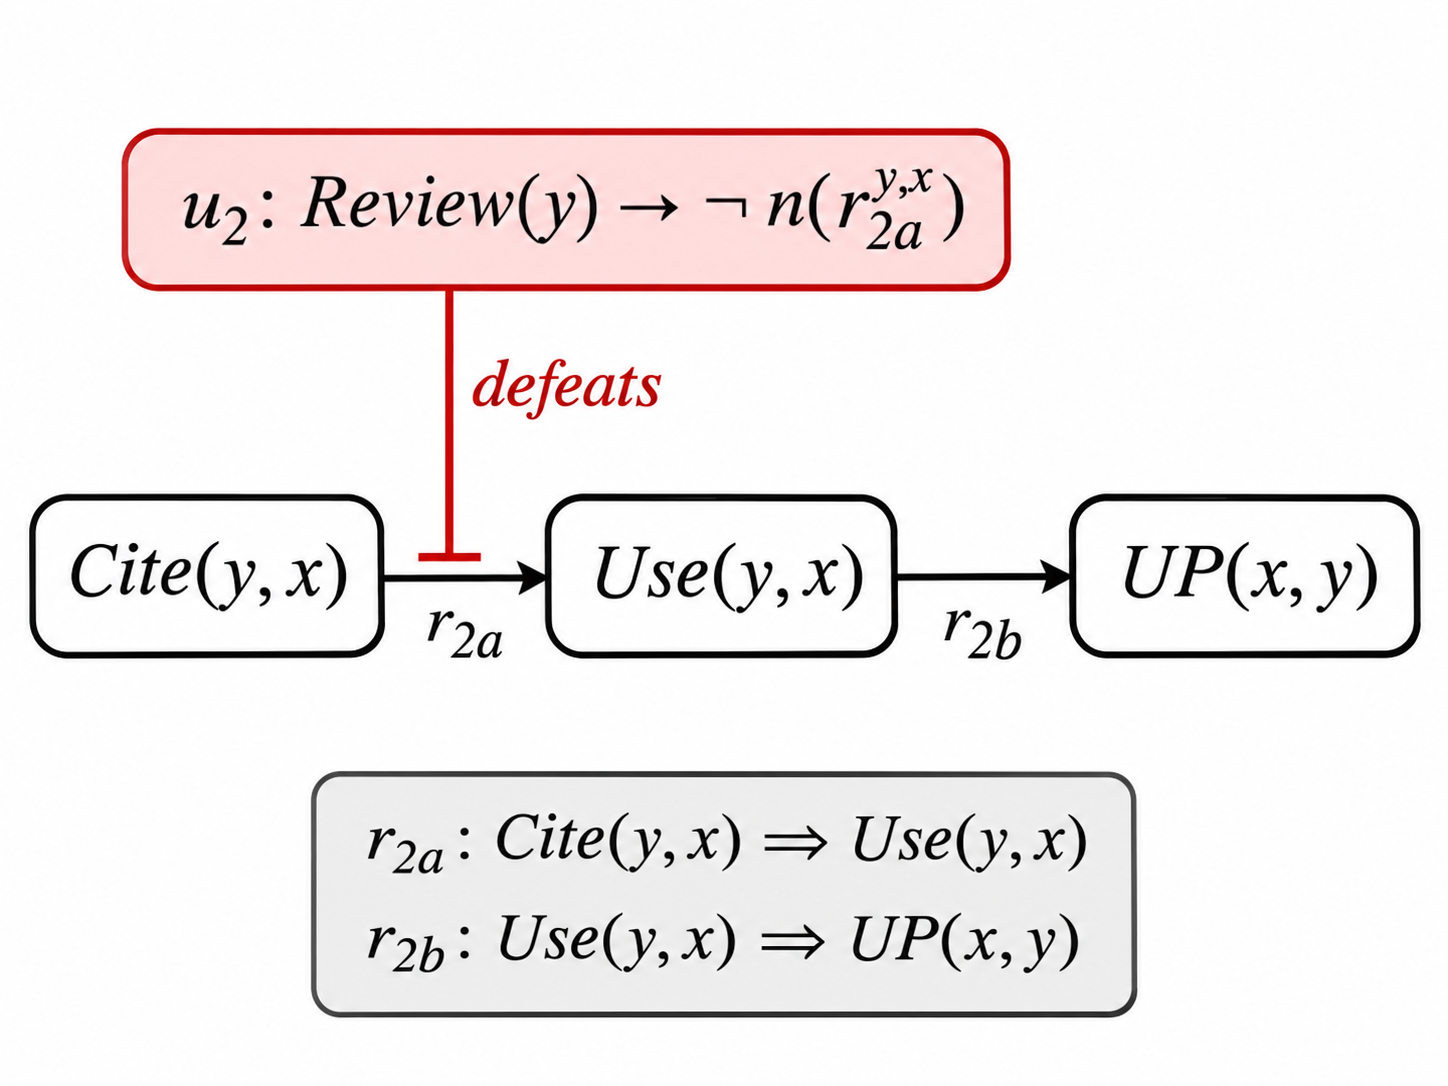
\includegraphics[width=\linewidth]{img/Review Defeat Diagram.png}\\[5pt]


\end{minipage}
\par\vspace{16pt}{\color{ink}\hrule}\vspace{9pt}
{\large\bfseries Final verdict: not at risk}\par

\end{minipage}}
\par\vspace{10pt}{\footnotesize Based on the annotated dataset and Chapter 6 prototype. Justifications and verdicts reproduce the saved Chapter 6 CSV results.}

\newpage
{\small\color{ink}CHAPTER 6 \quad COMPUTATIONAL PIPELINES}\par\vspace{12pt}
\fcolorbox{ink}{white}{\begin{minipage}{\dimexpr\linewidth-2\fboxsep-2\fboxrule\relax}
{\Large\bfseries Assessment Card}\par
\textbf{Lomas (2014)}\par\textit{$^1$H NMR spectra of alcohols and diols in chloroform: DFT/GIAO calculation of chemical shifts}\par
{\small DOI: \nolinkurl{10.1002/mrc.4130}}\par
\vspace{8pt}{\color{ink}\hrule}\vspace{12pt}
\begin{minipage}[t]{0.46\linewidth}\vspace{0pt}
\field{Justifications}
Publication lomas\_2014\_<sup>1</sup> (DOI: 10.1002/mrc.4130) is judged as \textbf{not at risk} of unreliability propagation because all citations to the WJH protocol appear in the introduction. This suggests that the protocol is cited as background information rather than used to conduct the research. However, this inference is defeasible: we identified two counterexamples previously in which all citations appeared in the introduction, but the citation text indicated use of the protocol.
\end{minipage}\hfill
\begin{minipage}[t]{0.49\linewidth}\vspace{0pt}
\field{Reasoning visualization}
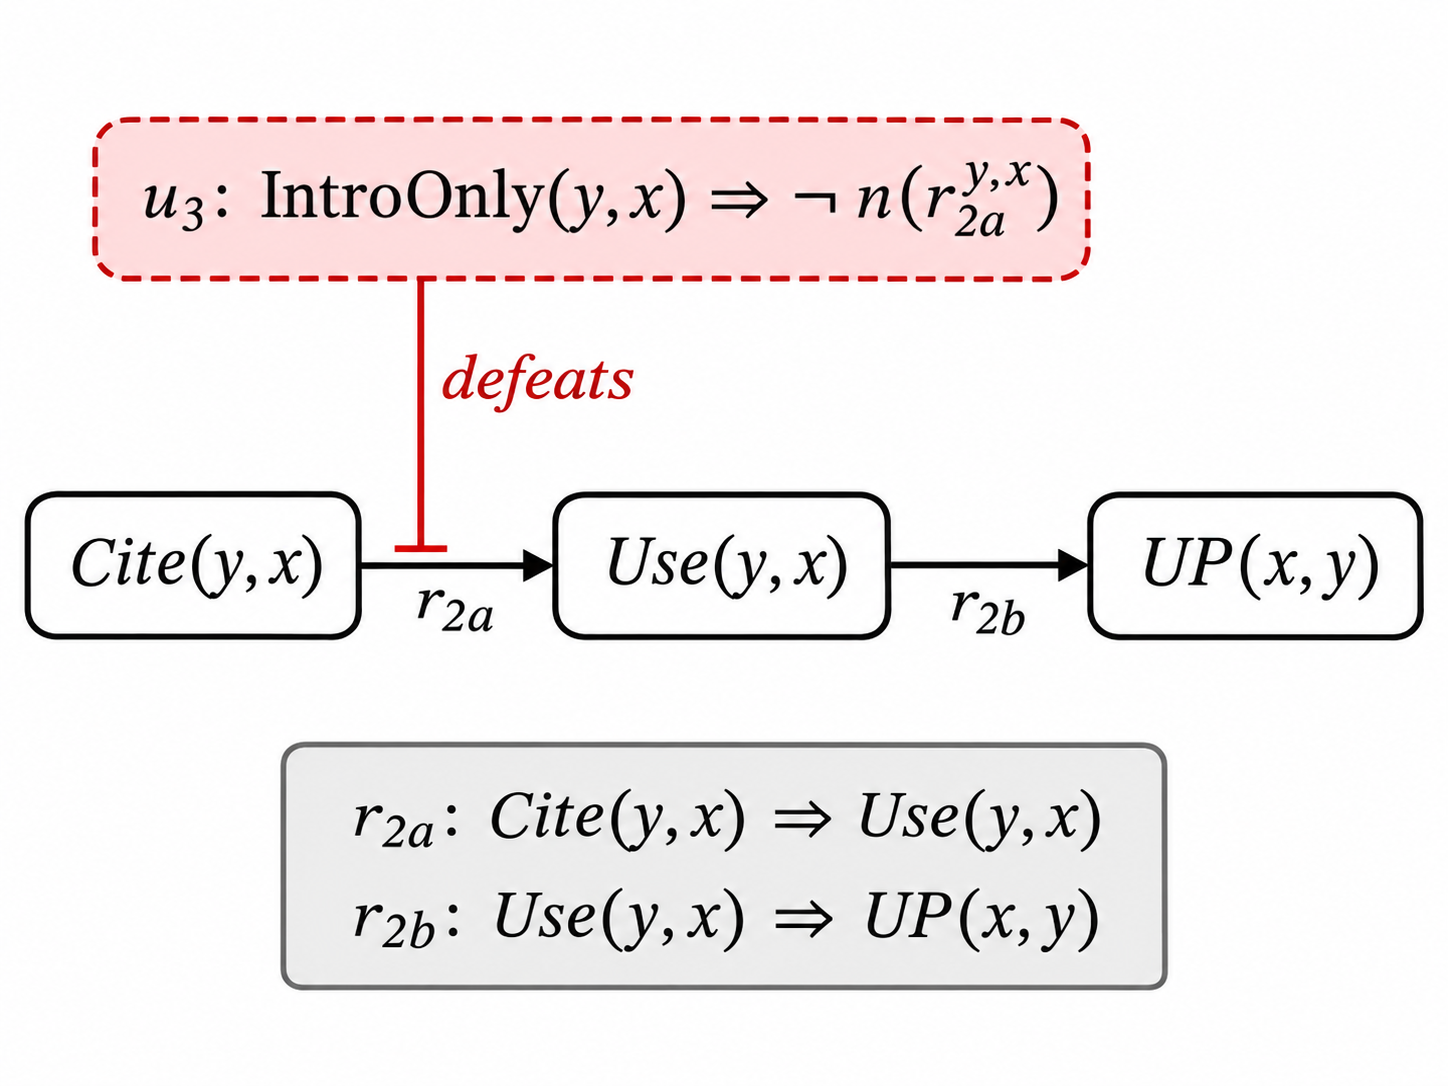
\includegraphics[width=\linewidth]{img/IntroOnly Defeat Diagrm.png}\\[5pt]


\end{minipage}
\par\vspace{16pt}{\color{ink}\hrule}\vspace{9pt}
{\large\bfseries Final verdict: not at risk}\par

\end{minipage}}
\par\vspace{10pt}{\footnotesize Based on the annotated dataset and Chapter 6 prototype. Justifications and verdicts reproduce the saved Chapter 6 CSV results.}

\newpage
{\small\color{ink}CHAPTER 6 \quad COMPUTATIONAL PIPELINES}\par\vspace{12pt}
\fcolorbox{ink}{white}{\begin{minipage}{\dimexpr\linewidth-2\fboxsep-2\fboxrule\relax}
{\Large\bfseries Assessment Card}\par
\textbf{Matsuo et al. (2017)}\par\textit{Structural Revision and Biomimetic Synthesis of Goupiolone B}\par
{\small DOI: \nolinkurl{10.1002/anie.201706532}}\par
\vspace{8pt}{\color{ink}\hrule}\vspace{12pt}
\begin{minipage}[t]{0.46\linewidth}\vspace{0pt}
\field{Justifications}
Publication matsuo\_2017\_structural (DOI: 10.1002/anie.201706532) is judged to remain \textbf{at risk} of unreliability propagation because neither the publication metadata, bibliography, nor the section headings under which citations appear provide a reason to defeat the inference from citation to unreliability propagation. This judgment is defeasible: additional evidence, including the content of citation contexts, may warrant revising it.
\end{minipage}\hfill
\begin{minipage}[t]{0.49\linewidth}\vspace{0pt}
\field{Reasoning visualization}
\vspace{30pt}\colorbox{wash}{\begin{minipage}{0.86\linewidth}\centering\vspace{16pt}No identified defeater\par\vspace{12pt}$\mathrm{Cite}(y,x)\Rightarrow\mathrm{UP}(x,y)$\par\vspace{12pt}Default inference remains defeasible.\vspace{16pt}\end{minipage}}

\end{minipage}
\par\vspace{16pt}{\color{ink}\hrule}\vspace{9pt}
{\large\bfseries Final verdict: at risk}\par

\end{minipage}}
\par\vspace{10pt}{\footnotesize Based on the annotated dataset and Chapter 6 prototype. Justifications and verdicts reproduce the saved Chapter 6 CSV results.}

\newpage
{\small\color{ink}CHAPTER 6 \quad COMPUTATIONAL PIPELINES}\par\vspace{12pt}
\fcolorbox{ink}{white}{\begin{minipage}{\dimexpr\linewidth-2\fboxsep-2\fboxrule\relax}
{\Large\bfseries Assessment Card}\par
\textbf{Kim et al. (2020)}\par\textit{Structure elucidation of small organic molecules by contemporary computational chemistry methods}\par
{\small DOI: \nolinkurl{10.1007/s12272-020-01277-4}}\par
\vspace{8pt}{\color{ink}\hrule}\vspace{12pt}
\begin{minipage}[t]{0.46\linewidth}\vspace{0pt}
\field{Justifications}
Publication kim\_2020\_structure (DOI: 10.1007/s12272-020-01277-4) is judged as \textbf{not at risk} of unreliability propagation because it cites either the paper reporting the code glitch (Neupane et al., 2019) or the addendum (Willoughby et al., 2020). Such a citation suggests that the authors were aware of the glitch and were therefore unlikely to carry its effects into their own work. This inference is defeasible: further evidence could lead us to revise the classification.

Publication kim\_2020\_structure (DOI: 10.1007/s12272-020-01277-4) is judged as \textbf{not at risk} of unreliability propagation because it is a review article. Review articles generally discuss existing research rather than execute computational procedures such as the WJH protocol. Review status therefore provides a reason not to infer that the authors used the protocol merely because they cited it.
\end{minipage}\hfill
\begin{minipage}[t]{0.49\linewidth}\vspace{0pt}
\field{Reasoning visualization}
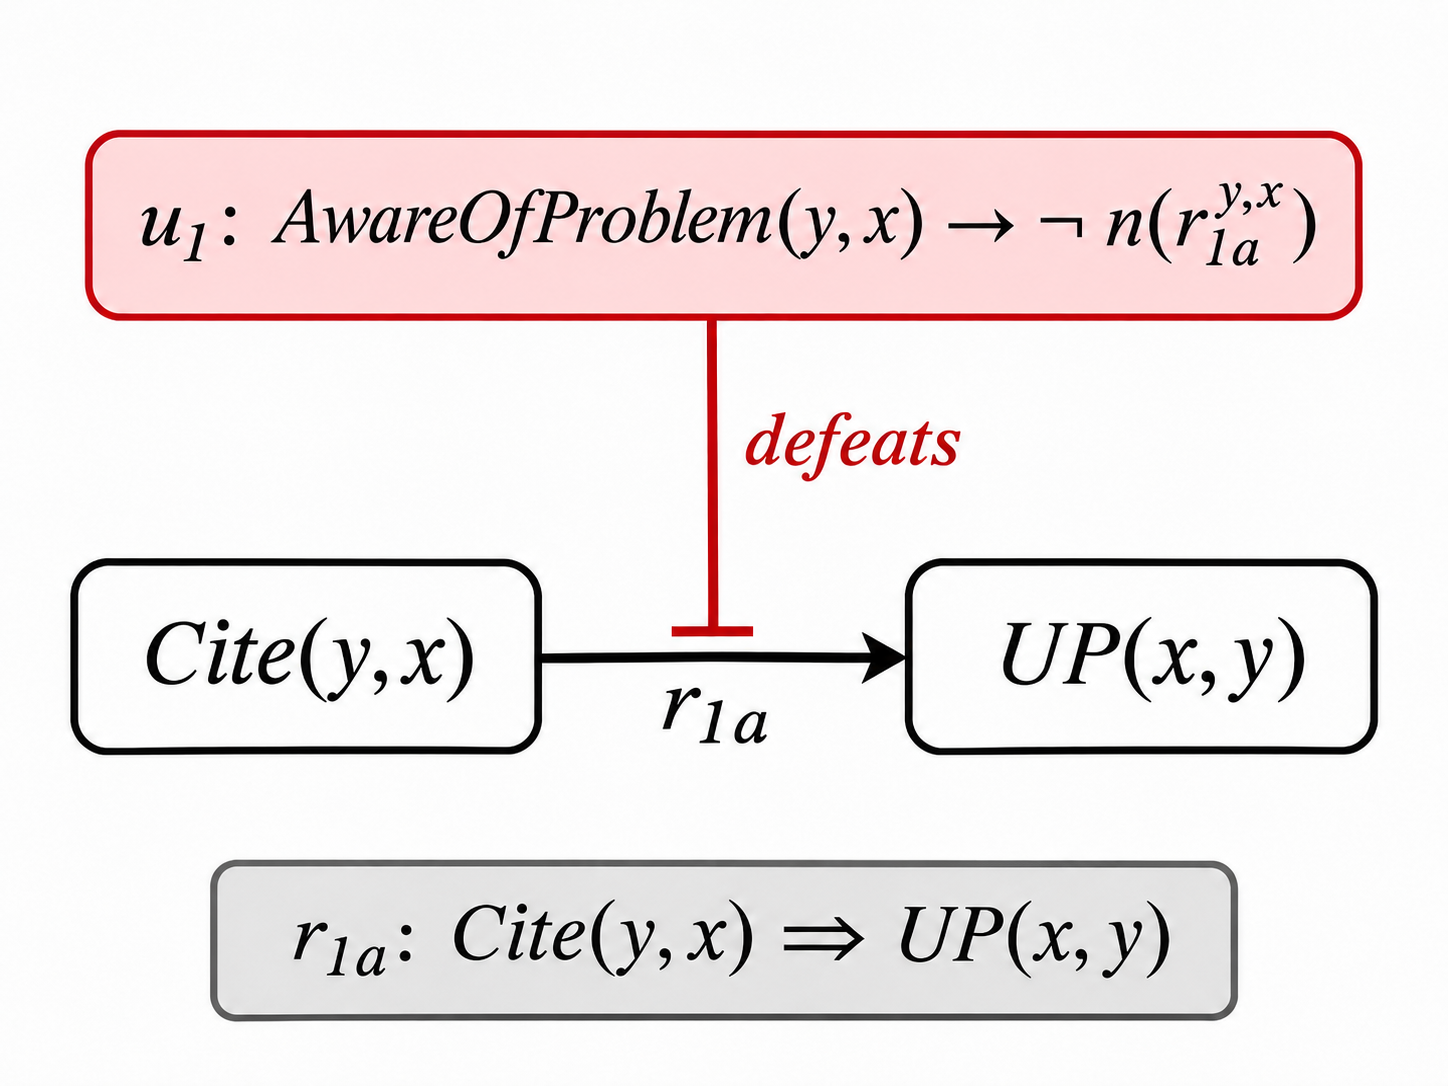
\includegraphics[width=0.91\linewidth]{img/AwareOfProblem Defeat Diagram.png}\\[5pt]
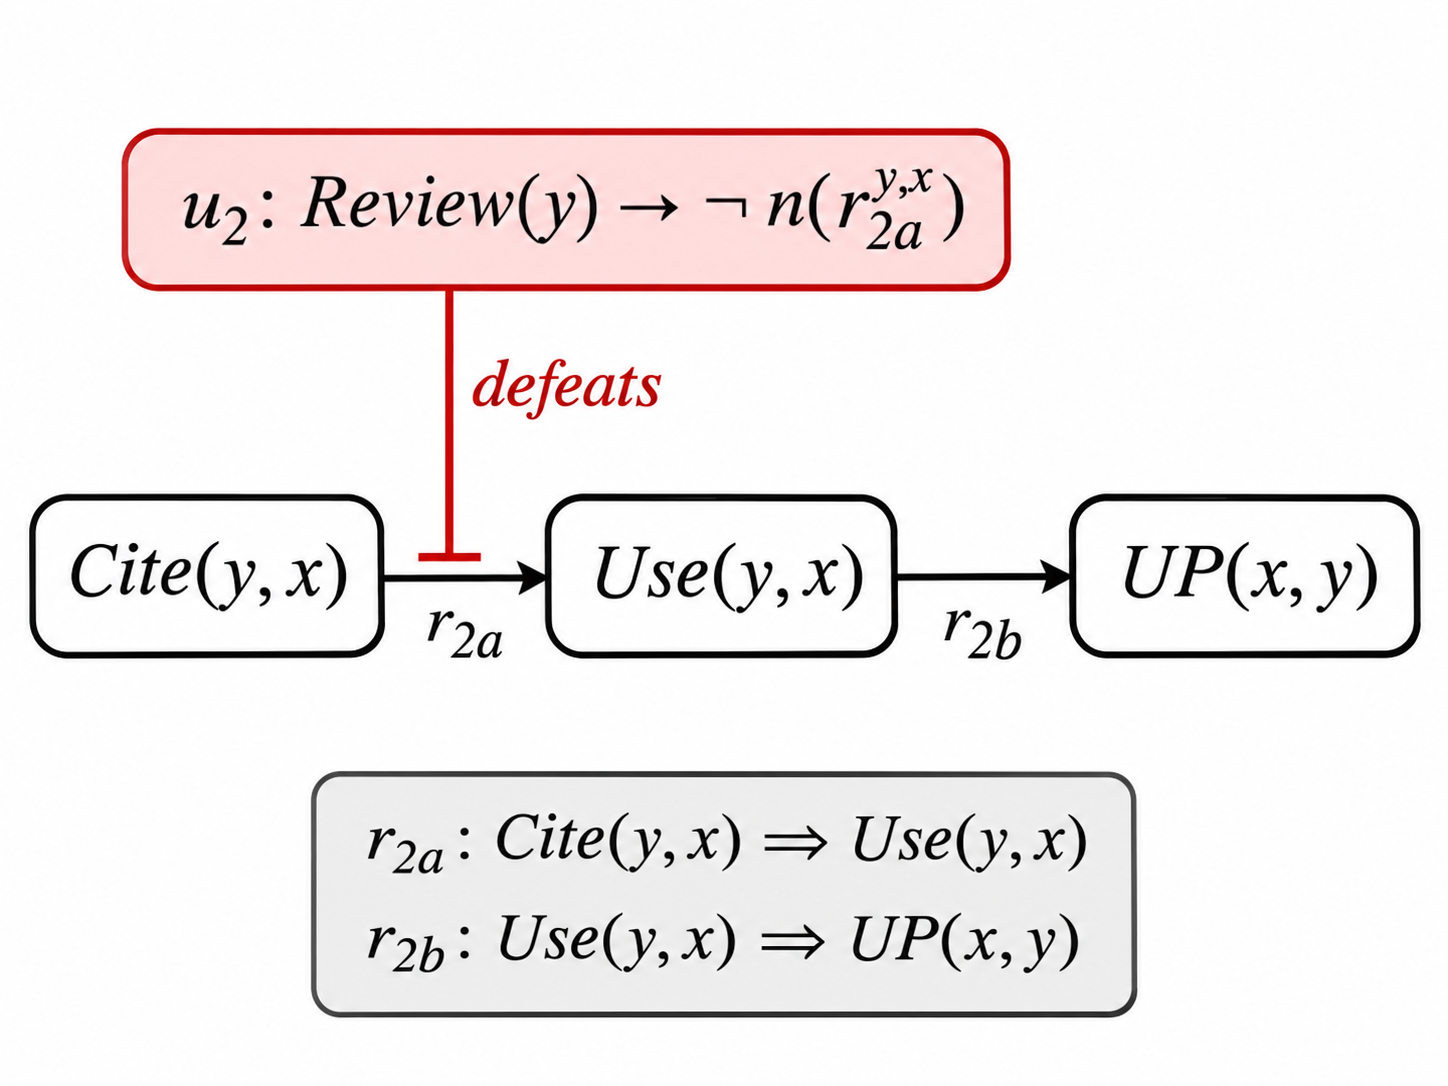
\includegraphics[width=0.91\linewidth]{img/Review Defeat Diagram.png}\\[5pt]


\end{minipage}
\par\vspace{16pt}{\color{ink}\hrule}\vspace{9pt}
{\large\bfseries Final verdict: not at risk}\par

\end{minipage}}
\par\vspace{10pt}{\footnotesize Based on the annotated dataset and Chapter 6 prototype. Justifications and verdicts reproduce the saved Chapter 6 CSV results.}

\end{document}
